% Evaluation criterion:
%- Language and use of figures
%- Clarity of the problem statement
%- Overall document structure
%- Depth of understanding for the field of computer architecture
%- Depth of understanding of the investigated problem

\section{Prefetcher Description}
\label{sec:prefetcherDescription}

In our paper, we will consider four different prefetching strategies,
each taken from a separate category of prefetchers identified in
Grannas' paper (reference needed). The first two prefetchers are address based, and does not need any information about the program counter. The latter two prefetchers both needs to know the program counter. 

\subsection{Address based stride prefetcher}
\label{sec:stridePrefetcher}
The address based stride prefetcher (ABSP) is a simplified version of the Stride Directory Prefetcher. The ABSP is based on the fact that memory accesses
often follow a stride-n pattern (where n is the number of addresses between
the accessed addressess). When accessing the members of an
array, or iterating through a loop, most of the memory accesses will
follow a stride-n pattern. An example can be shown in figure~\ref{fig:stride}.

\begin{figure}[H]
\label{fig:stride}
\centerline{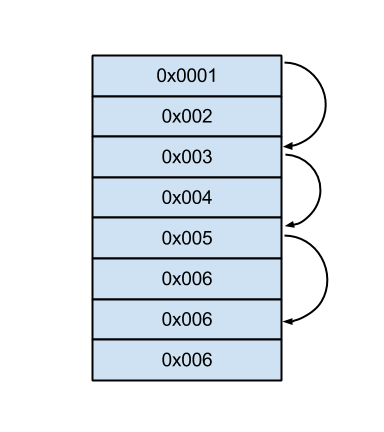
\includegraphics[scale=0.5]{./figures/stride}}
\caption{A memory access pattern with a stride of n=2}
\end{figure}

The ABSP keeps track of the last accessed address, what the delta of the addresses in the current stride is, and
also keeps track of for how long the current stride has been
ongoing. Compared to the Stride Directory Prefetcher, ABSP only requires a costant amount of memory (only the last accessed address is saved) and has a low degree of complexity.

For each memory access, the memory address is compared to the last
memory address. If the current stride value corresponds to the
difference, the number of current strides is updated. If the number of
current strides is greater than or equal to the required/configured
amunt of strides, a prefetched address is returned.  

The prefetchers can be configured by tweaking two variables;
the amount of strides that needs to be discovered before
the prefetcher will react on a memory access, and how many addresses it should prefetch once it is decided that it should prefetch.


% !TEX root = ../main.tex
\subsection{Markov Prefetcher}
\label{sec:markovPrefetcher}
The markov prefetcher, as described in \cite{Grannas}, is an address based prefetcher. It remembers past sequences of memory misses, and utilizes heuristics on these sequences to predict future memory accesses.

As shown in \cite{Joseph}, it utilizes a directed graph with nodes representing cache blocks, and weighted edges representing the probability that the successor node will be accessed after the predecessor node (see figure \ref{fig:markov}). The weight of the edges is determined by how often the cache block an edge points to is accessed directly after the node the edge is pointing from. For each memory access, the edge corresponding to the current transition needs to be updated. 

When predicting the next sequence of addresses, the markov prefetcher follows the most probable path through the graph. Configuring the markov prefetcher would allow you to decide how many addresses it should prefetch, when to create a new edge between two nodes, when to delete an edge and when to delete a node.

Looking at figure \ref{fig:markov}, if two addresses were to be prefetched, and \emph{0x0001} was the current node, then addresses \emph{0x0002} and \emph{0x0003} would be prefetched.

\begin{figure}[H]
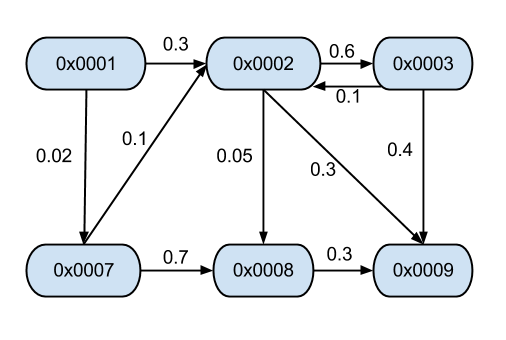
\includegraphics[scale=0.5]{./figures/markov}
\caption{\label{fig:markov}A snippet of a possible weighted graph used by the markov prefetcher.}
\end{figure}


\subsection{Global History Buffer Prefetcher}
\label{sec:ghbPcdcPrefetcher}

The global history buffer prefetcher is an instruction based
prefetching scheme, i.e. a prefetcher which uses the value of the
program counter at the memory access time to gather statistics about,
and from these predict, future memory accesses. In
this scheme, a data structure called Global History Buffer (GHB) is maintained. This data structure is a table whose elements are
addresses for which a cache miss has recently occurred, as well as a
pointer to the previous entry representing a miss
with the same program counter as the given miss. The
structure is illustrated in figure~\ref{fig:ghbStruct}.

\begin{figure}[ht]
  \centering
  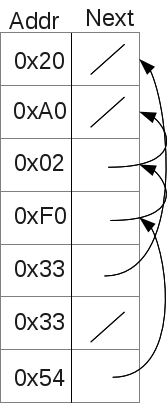
\includegraphics[scale=0.5]{figures/ghb_diag.png}
  \caption{\label{fig:ghbStruct} Structure of the GHB. Each table
    element contains two items: The requested address, and the
    previous cache miss caused by from the same program counter as
    this entry came from.}
\end{figure}

Complementary to this table, an index table is used to record the last
entry inserted into the GHB for a given program counter value. With
these two data structures, you can obtain the recent miss history for a
given load by traversing the linked list of table entries. There are
several ways to use this information to predict what addresses might
be needed in the future. We have decided to implement a version called
GHB/PCDC (Global History Buffer, Program Counter based with Delta
Correlation \cite{Grannas}). The idea is to extend the constant stride
prefetcher with the ability to recognize patterns of non-constant
stride accesses. Specifically, on a cache miss the offsets between
previous misses for the current program counter is computed and stored
in what is known as a delta table. An example of this is given in
figure~\ref{fig:deltaTableComp}. 

\begin{figure}[ht]
  \centering
  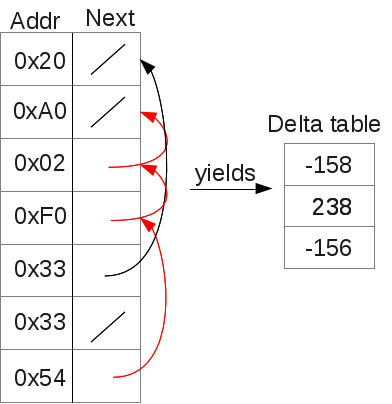
\includegraphics[scale=0.5]{figures/delta_table_comp.png}
  \caption{\label{fig:deltaTableComp} Computation of a delta table for
    a given miss, where the miss history is marked with red
    arrows. The four registered misses results in three delta values.}
\end{figure}

The delta table is then searched backwards for the previous occurrence
of the last two delta values. In the example in
figure~\ref{fig:deltaTableComp}, GHB searches for the delta values
--156 and --238. If these have not occurred previously, as they indeed
have not in this example, then GHB do not prefetch anything as it has
no information about the past. If they are found, however, GHB would prefetch
addresses according to the deltas which followed the previous delta
pair occurrence. 

An example of where this technique would improve upon the stride
prefetcher follows, as given in \cite{Nesbit}. Assume the program accesses the
first few columns of each row of a multidimensional array. This would
result in a few constant stride misses, followed by a miss with a
delta corresponding to the size of the remaining row. A stride directed
prefetcher would issue prefetches for the constant stride, which would
be unneeded when you start accessing the next row.
% Furthermore, if the number of columns accessed was small the stride
% prefetcher might not register the constant stride in time to
% actually perform any useful prefetches
In contrast, the delta correlating prefetcher would create a history
buffer which paid heed to the larger delta value. On subsequent misses
to the next row, it would look up in its history table that what
follows this large delta is actually a series of constant stride
misses. It could then start prefetching sensible addresses right away.

Another example would be code which traverses the same linked data
structure multiple times. Consider the following loop:
\begin{lstlisting}
  void f(list *l) {
    for (list *n = l; n; n = n->next) {
      process(n);
    }
  }
\end{lstlisting}
In particular, consider the end-of-loop statement {\lstinline|n =  n->next|}. 
Assuming a register {\lstinline|r1|} contained {\lstinline|n|}, this
would compile into something like the following:
\begin{lstlisting}
  ld r1, [r1, nextOffset] @ 1. Load the offset value
  ld r1, [r1]             @ 2. Load the next pointer
\end{lstlisting}
The second statement would access addresses with a delta value of the
elements of the list. So would the first statement, as the offset of
the {\lstinline|next|} field is constant in the data structure. In
fact, so should most loads and stores accessing {\lstinline|n|} in
{\lstinline|process|}, given that they do not occur within nested
loops. The first time {\lstinline|f|} is run there would be no
benefit, but if it is a function that is called a lot with the same
list then on future calls the first iterations should register the
start of the loop, and prefetch the addresses belonging to elements
further on in the list.

\subsection{Spatial Memory Streaming Prefetcher}
\label{sec:smsPrefetcher}

The Spatial Memory Streaming (SMS) Prefetcher is a spatial locality
prefetcher which ideas was first presented in \cite{SMS}, it tries to
exloit the relationship between a memory page, and a cache line.

Since a memory page is larger than a cache line, the memory page is
fragmented across several cache lines, and even though the page is in
memory, only parts of it may be in the cache.  When designing
operating systems and database management systems, the system designer
will optimize the design for the memory page size in order to limit
the amount of bandwidth and access to the disk. In order to achieve
this, large and complex data structures will have to be chunked up into
smaller and equal structures that fit into a single memory page.

When performing large scale operations on these data structures, for
example a database search, the program might sit in a loop while it
processes several of these page sized data structures. For instance,
while processing these pages the program might always access a page
header, a B-tree key-pointer and a pointer collection at the end of
the page. By recording the access pattern on a single page the pattern may
be used on multiple pages each time the program accesses a new page
with the same program counter and the same page offset.

\begin{figure}[H]
  \centering
  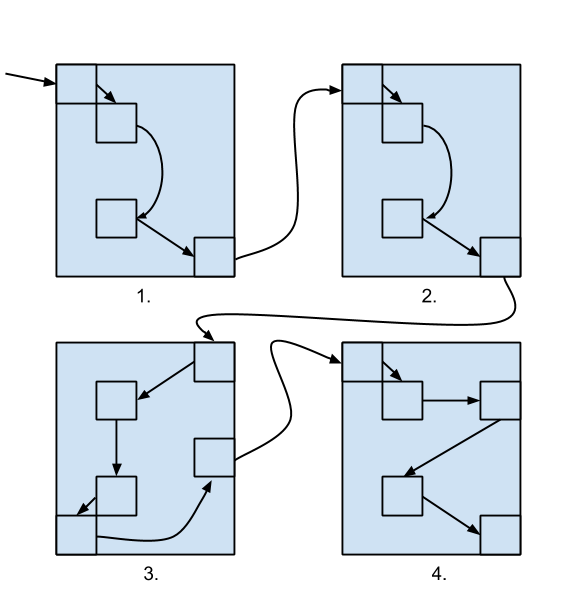
\includegraphics[scale=0.35]{./figures/sms_pattern.png}
  \caption{Cache blocks accessed across memory pages}
  \label{fig:sms_pattern}
\end{figure}

Figure \ref{fig:sms_pattern} shows the opportunities that SMS tries to exploit, here pages 1 and 2 have exactly the same access pattern. Page 4 has a similar entry point but differs from 1 and 2 in that it has one more cache block. Altought Page 3 has some similar blocks it differs in entry. SMS will exploit the pattern that was recorded on page 1 to prefetch the blocks in Page 2 and 4.

\subsubsection{How it works}
SMS uses two different tables in its implementation. The Active
Generation Table (AGT) which is used when recording spatial pattern,
and the Page History Table (PHT) which stores recorded patterns. 

A generation is the time over which SMS records access to a spatial
memory region. The spatial memory region is the collection of cache
lines the SMS considers as a larger memory structure and it emulates
the operating system memory page. The memory access that triggers a
generation is referred to as a trigger access and it is the first
access to memory region which is not currently being recorded in the
AGT. The generation ends when one of the accessed cache lines that
have been accessed during the generation is invalidated or evicted
from the cache.  When a generation ends it is transferred from the AGT
to the PHT if it has two or more accesses within the spatial
region. In order to make the implementation easier the AGT is divided
into two tables, the filter table and the accumulation table.  Upon a
trigger access the generation is first inserted into the filter table,
when the spatial region is accessed a second time, it is moved from
the filter table to the accumulation table. All subsequent accesses
updates the spatial pattern in the accumulation table.  An entry in
the AGT consist of a tag, which is the base address of the spatial
region, the program counter and the offset that triggered the
generation and a spatial bit pattern of the cache lines which has been
accessed during the generation. 

\begin{table}[htbp]
  \centering
  \begin{tabular}{| c | c |}
    \hline
    {\bf Access} & {\bf Action} \\ \hline
    A + 0 & Generation A [0001]\\ \hline
    A + 1 & Generation A [0011]\\ \hline
    A + 3 & Generation A [1011]\\ \hline
    B + 2 & Generation B [0100]\\ \hline
    C + 1 & Generation C [0010] \\ \hline
    evict A + 1 & Move Generation A to PHT\\ \hline
    A + 0 & Generation A' [0001]\\ \hline
    A + 2 & Generation A' [0101]\\ \hline
    B + 3 & Generation B [1100] \\ \hline
    invalidate B + 2 & Move Generation B to PHT\\ \hline
    evict C + 1 & Remove Generation C from AGT \\ \hline    
  \end{tabular}
  \caption{The lifetime of Generations}
  \label{tab:generation}
\end{table}
Table \ref{tab:generation} shows an access sequence and the
actions applied to the generations and their pattern in the AGT.

Upon a trigger access SMS searches the history table for a pattern
that can be used to predict which addresses will be accessed.  A PHT
entry has a tag which is the program counter and the spatial region
offset of the trigger access to the recorded generation, and the
recorded spatial pattern that was recorded during the generation.
When searching through the PHT the current program counter and spatial
region offset is compared to the PHT tag. If there is a match in the
PHT a set of predicted addresses is constructed from the spatial
region base address and the set of block offsets recorded in the
spatial pattern. These addresses is then put into a queue of memory
addresses to be streamed into the cache.

